%Metroplolis Beamer Theme: https://github.com/matze/mtheme
\documentclass[aspectratio=169, 10pt, dvipsnames]{beamer}
\usetheme{metropolis}
\usepackage{appendixnumberbeamer, lmodern, bookmark,fontawesome}
\usepackage{booktabs}
% \usepackage[sorting=none]{biblatex}
\usepackage[scale=2]{ccicons}
\usepackage{pgfplots}
\usepgfplotslibrary{dateplot}
\usepackage{xspace}
\newcommand{\themename}{\textbf{\textsc{metropolis}}\xspace}
\usepackage{bbm}
\usepackage{tikz, graphicx}
\usepackage{multicol}
% \usepackage[dvipsnames]{xcolor}
\usepackage{animate}
\usepackage{scalerel,xparse}
\usepackage{amsmath}
\usepackage{subfig}
\usepackage[style=british]{csquotes}
\usepackage{pgfplots}
\usepackage[outline]{contour}
\usepackage{minted}
\usepackage[font=tiny]{caption}


\newcommand*\colourcheck[1]{%
  \expandafter\newcommand\csname #1check\endcsname{\textcolor{#1}{\ding{52}}}%
}
\newcommand{\ra}[1]{\renewcommand{\arraystretch}{#1}}                % Make distance in tables better
\colourcheck{blue}
\contourlength{1.2pt}

\title{Building a library to evaluate generative protein models}
% \subtitle{Lab Update}
\date{\today}
\author{Philip Hartout}

% \titlegraphic{\hfill\includegraphics[height=1.5cm]{logo.pdf}}

\hypersetup{
  colorlinks=true,
  linkcolor=orange,
  filecolor=orange,
  urlcolor=orange,
}
% Configuration of TikZ. These packages are primarily required for
% preparing the overview figure.

\def\signed #1{{\leavevmode\unskip\nobreak\hfil\penalty50\hskip1em
  \hbox{}\nobreak\hfill #1%
  \parfillskip=0pt \finalhyphendemerits=0 \endgraf}}

\newsavebox\mybox
\newenvironment{aquote}[1]
  {\savebox\mybox{#1}\begin{quote}\openautoquote\hspace*{-.7ex}}
  {\unskip\closeautoquote\vspace*{1mm}\signed{\usebox\mybox}\end{quote}}

\titlegraphic{%
  
\includegraphics[width=.2\textwidth]{figures/mlcb-transparent.png}\hfill
  
\includegraphics[width=.2\textwidth]{figures/dbsse-transparent.png}\hfill
  
\includegraphics[width=.2\textwidth]{figures/eth-transparent.png}
}

\makeatletter
\setbeamertemplate{title page}{
  \begin{minipage}[b][\paperheight]{\textwidth}
    \vfill%
    \ifx\inserttitle\@empty\else\usebeamertemplate*{title}\fi
    \ifx\insertsubtitle\@empty\else\usebeamertemplate*{subtitle}\fi
    \usebeamertemplate*{title separator}
    \ifx\beamer@shortauthor\@empty\else\usebeamertemplate*{author}\fi
    \ifx\insertdate\@empty\else\usebeamertemplate*{date}\fi
    \ifx\insertinstitute\@empty\else\usebeamertemplate*{institute}\fi
    \vfill
    \ifx\inserttitlegraphic\@empty\else\inserttitlegraphic\fi
    \vspace*{1cm}
  \end{minipage}
}
\makeatother

\usetikzlibrary{shapes.geometric,arrows,calc,positioning,backgrounds,decorations.pathreplacing,
  decorations.pathmorphing, shapes,matrix,shapes.symbols,chains,patterns,fit,scopes,external
}

\tikzstyle{orangebox} = [rectangle, rounded corners, minimum width=2cm, minimum
height=0.5cm, draw=black, fill=YellowOrange!60, very thick]
\tikzstyle{bluebox} = [rectangle, rounded corners, minimum width=2cm, minimum height=0.5cm, draw=black, fill=blue!40]
\tikzstyle{arrow} = [thick,->,>=stealth]
\def\xlist{4}
\def\ylist{4}
\newcommand{\fillrandomly}[7]{
  \pgfmathsetmacro\diameter{#3*2}
  % \draw (0,0) rectangle (#1,#2);
  \foreach \i in {1,...,#4}{
    \pgfmathsetmacro\x{rnd*#1}
    \pgfmathsetmacro\y{rnd*#2}
    \xdef\collision{0}
    \foreach \element [count=\i] in \xlist{
      \pgfmathtruncatemacro\j{\i-1}
      \pgfmathsetmacro\checkdistance{ sqrt( ({\xlist}[\j]-(\x))^2 + ({\ylist}[\j]-(\y))^2 ) }
      \ifdim\checkdistance pt<\diameter pt
        \xdef\collision{1}
        \breakforeach
      \fi
    }
    \ifnum\collision=0
      \xdef\xlist{\xlist,\x}
      \xdef\ylist{\ylist,\y}
      \draw [#5, fill=#5] (\x + #6,\y+ #7) circle [radius=#3];
    \fi

  }
}
\newcommand\arrowfromto[5][blue]{%
  \draw[#1] #2 -- ( $ #2!#4!#3 $ ) node [midway, sloped, above] {#5}}

\setminted[python]{fontsize=\tiny}

\begin{document}

% define gaussian pdf and cdf
\pgfmathdeclarefunction{gauss}{3}{%
  \pgfmathparse{1/(#3*sqrt(2*pi))*exp(-((#1-#2)^2)/(2*#3^2))}%
}
\pgfmathdeclarefunction{cdf}{3}{%
  \pgfmathparse{1/(1+exp(-0.07056*((#1-#2)/#3)^3 - 1.5976*(#1-#2)/#3))}%
}
\pgfmathdeclarefunction{fq}{3}{%
  \pgfmathparse{1/(sqrt(2*pi*#1))*exp(-(sqrt(#1)-#2/#3)^2/2)}%
}
\pgfmathdeclarefunction{fq0}{1}{%
  \pgfmathparse{1/(sqrt(2*pi*#1))*exp(-#1/2))}%
}

\colorlet{mydarkblue}{blue!30!black}

% to fill an area under function
\usepgfplotslibrary{fillbetween}

\pgfplotsset{compat=1.12} % TikZ coordinates <-> axes coordinates
% https://tex.stackexchange.com/questions/240642/add-vertical-line-of-equation-x-2-and-shade-a-region-in-graph-by-pgfplots

% plot aspect ratio
% \def\axisdefaultwidth{8cm}
% \def\axisdefaultheight{6cm}

% number of sample points
\def\N{50}

\maketitle


\begin{frame}[fragile]{Introduction}
  \begin{minipage}{0.7\textwidth}
  \begin{figure}
    \centering
    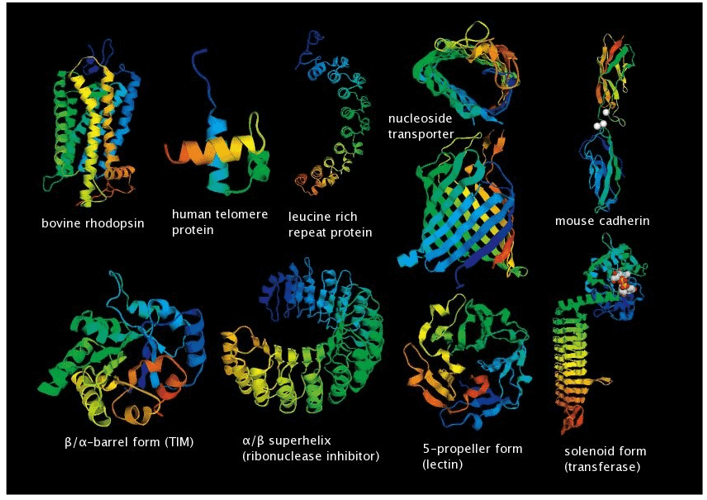
\includegraphics[width=\textwidth]{./figures/structures.png}
  \end{figure}
\end{minipage}
\hfill
\begin{minipage}{0.25\textwidth}
  \small Proteins are diverse.

  \pause\small Support all functions for life.
\end{minipage}
\end{frame}

\begin{frame}[fragile]{Generative Protein Modelling}
  \begin{minipage}{0.48\textwidth}
    \begin{alert}{Proteins}
      \begin{itemize}
        \pause \item well-defined (sequence)
        \pause \item large databases
      \end{itemize}
    \end{alert}

    \pause\begin{alert}{Generative Model}
      \begin{itemize}
        \pause\item captures $P(X)$
        \pause\item generate samples following  $P(X)$
      \end{itemize}
    \end{alert}
    \begin{center}
    \begin{minipage}{0.7\textwidth}
    \pause\begin{figure}
      \centering
      \begin{tikzpicture}
        \message{Cumulative probability^^J}

        \def\B{11};
        \def\Bs{3.0};
        \def\xmax{\B+3.2*\Bs};
        \def\ymin{{-0.1*gauss(\B,\B,\Bs)}};
        \def\h{0.07*gauss(\B,\B,\Bs)};
        \def\a{\B-0.8*\Bs};

        \begin{axis}[every axis plot post/.append style={
            mark=none,domain={-0.05*(\xmax)}:{1.08*\xmax},samples=\N,smooth},
          xmin={-0.1*(\xmax)}, xmax=\xmax,
          ymin=\ymin, ymax={1.1*gauss(\B,\B,\Bs)},
          axis lines=middle,
          % axis line style=thick,
          enlargelimits=upper, % extend the axes a bit to the right and top
          ticks=none,
          % xlabel=$x$,
          every axis x label/.style={at={(current axis.right of origin)},anchor=north},
          width=0.6*\textwidth, height=0.9\textwidth,
          y=120pt,
          clip=false
          ]

          % PLOTS
          \addplot[black,name path=B] {gauss(x,\B,\Bs)};

          % % FILL
          % \path[name path=xaxis]
          % (0,0) -- (\pgfkeysvalueof{/pgfplots/xmax},0);
          % \addplot[blue!25] fill between[of=xaxis and B, soft clip={domain=-1:{\a}}];

          % % LINES
          % \addplot[mydarkblue,dashed,thick]
          % coordinates {({\a},{1.2*gauss(\a,\B,\Bs)}) ({\a},{-\h})}
          % node[mydarkblue,below=-2pt] {$a$};
          % \node[mydarkblue,above right] at ({\B+\Bs},{1.2*gauss(\B+\Bs,\B,\Bs)}) {$f(x)$};
          % \node[blue!60!black,above left] at ({0.85*(\a)},{1.0*gauss(0.85*(\a),\B,\Bs)}) {$P(X\leq a)$};

        \end{axis}
      \end{tikzpicture}
      \hfill
      \begin{tikzpicture}
        \node (0) at (0,0) {};
        \draw [-latex](0,0.25) -- (0.8,0.25);
      \end{tikzpicture}
      \hfill
      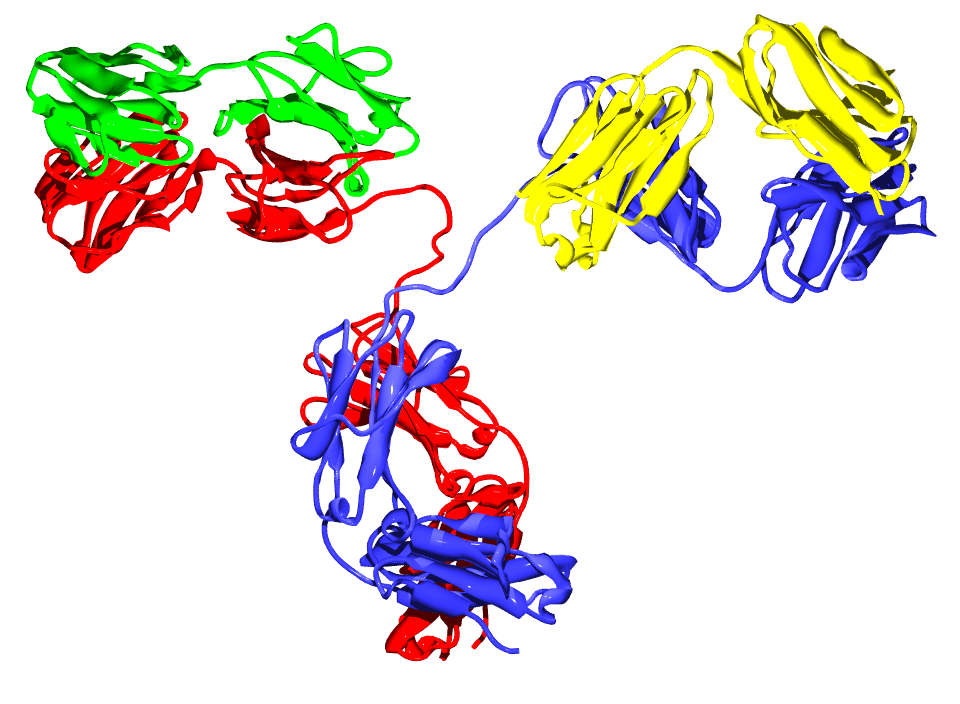
\includegraphics[width=0.3\textwidth]{./figures/ribbon.png}
    \end{figure}
    \end{minipage}
  \end{center}

  \end{minipage}
  \hfill
  \begin{minipage}{0.48\textwidth}
    \pause\begin{alert}{Evaluation Problem}
      \begin{itemize}
        \pause\item Are the generated and empirical data distributions the same?
      \end{itemize}
    \end{alert}

    \begin{figure}
    \centering
      \begin{tikzpicture}[scale=0.7]
  \message{Test statistics^^J}

  \def\q{6.3};
  \def\B{8.3};
  \def\S{4};
  \def\Bs{1.0};
  \def\Ss{1.5};
  \def\xmax{\B+3.2*\Bs};
  \def\ymin{{-0.15*gauss(\B,\B,\Bs)}};

  \begin{axis}[every axis plot post/.append style={
               mark=none,domain={-0.05*(\xmax)}:{1.08*\xmax},samples=\N,smooth},
               xmin={-0.1*(\xmax)}, xmax=\xmax,
               ymin=\ymin, ymax={1.1*gauss(\B,\B,\Bs)},
               axis lines=middle,
               axis line style=thick,
               enlargelimits=upper, % extend the axes a bit to the right and top
               ticks=none,
               % xlabel=$t$,
               every axis x label/.style={at={(current axis.right of origin)},anchor=north west},
               width=\textwidth, height=0.7\textwidth,
               y=210pt
              ]

    % PLOTS
    \addplot[PineGreen, name path=B,thick] {gauss(x,\B,\Bs)};
    \addplot[YellowOrange,  name path=S,thick] {gauss(x,\S,\Ss)};
    % \addplot[black,dashed,thick]
    %   coordinates {(\q, {0.95*gauss(\B,\B,\Bs)}) (\q, \ymin)}
    %   node[below=3pt,anchor=south west] {$t_\text{cut}$};

    % FILL
    % \path[name path=xaxis]
    %   (0,0) -- (\pgfkeysvalueof{/pgfplots/xmax},0); %\pgfkeysvalueof{/pgfplots/xmin}
    % \addplot[white!50!blue] fill between[of=xaxis and B, soft clip={domain=0:\q}];
    % \addplot[white!50!red]  fill between[of=xaxis and S, soft clip={domain=\q:\xmax}];

    % % LABELS
    \node[above=2pt,     PineGreen] at (   \B,  {gauss(\B,\B,\Bs)}) {Empirical};
    \node[above left=2pt,YellowOrange]  at (1.2*\S,{gauss(\S,\S,\Ss)}) {Generated};
    % \node[below=2pt] at ($(0,0)!0.3!(\q,0)$)     {REJECT};
    % \node[below=2pt] at ($(\q,0)!0.7!(\xmax,0)$) {ACCEPT};

  \end{axis}
\end{tikzpicture}

  \end{figure}

\end{minipage}
% \begin{figure}
%   \centering
%   \includegraphics[width=.6\textwidth]{./figures/comparison.png}
% \end{figure}
\end{frame}

% \begin{frame}[standout]
%   What makes a good protein?
% \end{frame}

\begin{frame}[fragile]{Maximum Mean Discrepancy (MMD)}
  \begin{figure}
    \centering
      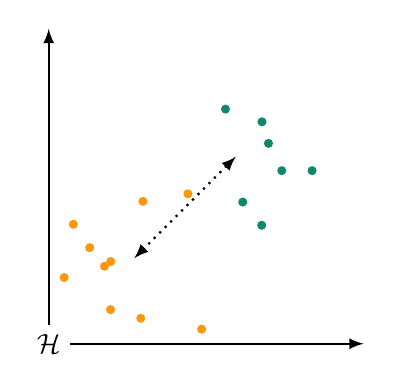
\begin{tikzpicture}
        \pgfmathsetseed{2}
        \node (0) at (0,0) {$\mathcal{H}$};
        \node (a) at (0,2) {};
        \node (b) at (2,0) {};
        \node (c) at (2.5,2.5) {};
        \fillrandomly{2}{2}{0.05}{10}{YellowOrange}{0}{0};
        \fillrandomly{2}{2}{0.05}{10}{PineGreen}{1.5}{1.5};
        \arrowfromto[-latex,black, thick]{(0)}{(a)}{4cm}{};
        \arrowfromto[-latex,black, thick]{(0)}{(b)}{4cm}{};
        \arrowfromto[latex-latex,dotted,black, thick]{(c)}{(0)}{2cm}{};
      \end{tikzpicture}
    \end{figure}
    \begin{center}
      \small MMD captures the distance between 2 sets on \emph{any} RKHS $\mathcal{H}$.
    \end{center}

\end{frame}


\begin{frame}[fragile]{Maximum Mean Discrepancy (MMD) -- continued}
  \begin{minipage}{0.68\textwidth}
  \pause\small Currently accepted method to evaluate generative GNNs.
  \pause\begin{figure}
    \centering
    \scalebox{0.75}{
      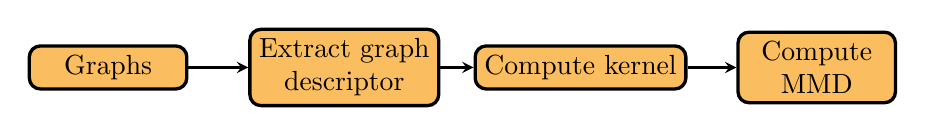
\begin{tikzpicture}[align=center, node distance=1.5cm, align=center]
        \node (graphs) [orangebox] {Graphs};
        \node (descriptor) [orangebox, right of=graphs, xshift=1.5cm] {Extract graph\\ descriptor};
        \draw [arrow] (graphs) -- (descriptor);
        \node (kernel) [orangebox, right of=descriptor, xshift=1.5cm] {Compute kernel};
        \draw [arrow] (descriptor) -- (kernel);
        \node (mmd) [orangebox, right of=kernel, xshift=1.5cm] {Compute \\MMD};
        \draw [arrow] (kernel) -- (mmd);
      \end{tikzpicture}
    }
  \end{figure}
    \pause\small It's possible to leverage decades of kernel research!\\
    \pause Both a
    \textcolor{PineGreen}{blessing} and a \textcolor{YellowOrange}{curse}:
    \begin{itemize}
      \pause\item[\textcolor{PineGreen}{Blessing}] Flexibility, Computation on
      multiple representations
      \pause\item[\textcolor{YellowOrange}{Curse}] Instability (see O'Bray et
      al (2021)), hyperparameter tuning.
    \end{itemize}

  \end{minipage}
  \hfill
  \begin{minipage}{0.28\textwidth}
  \begin{figure}
    \centering
    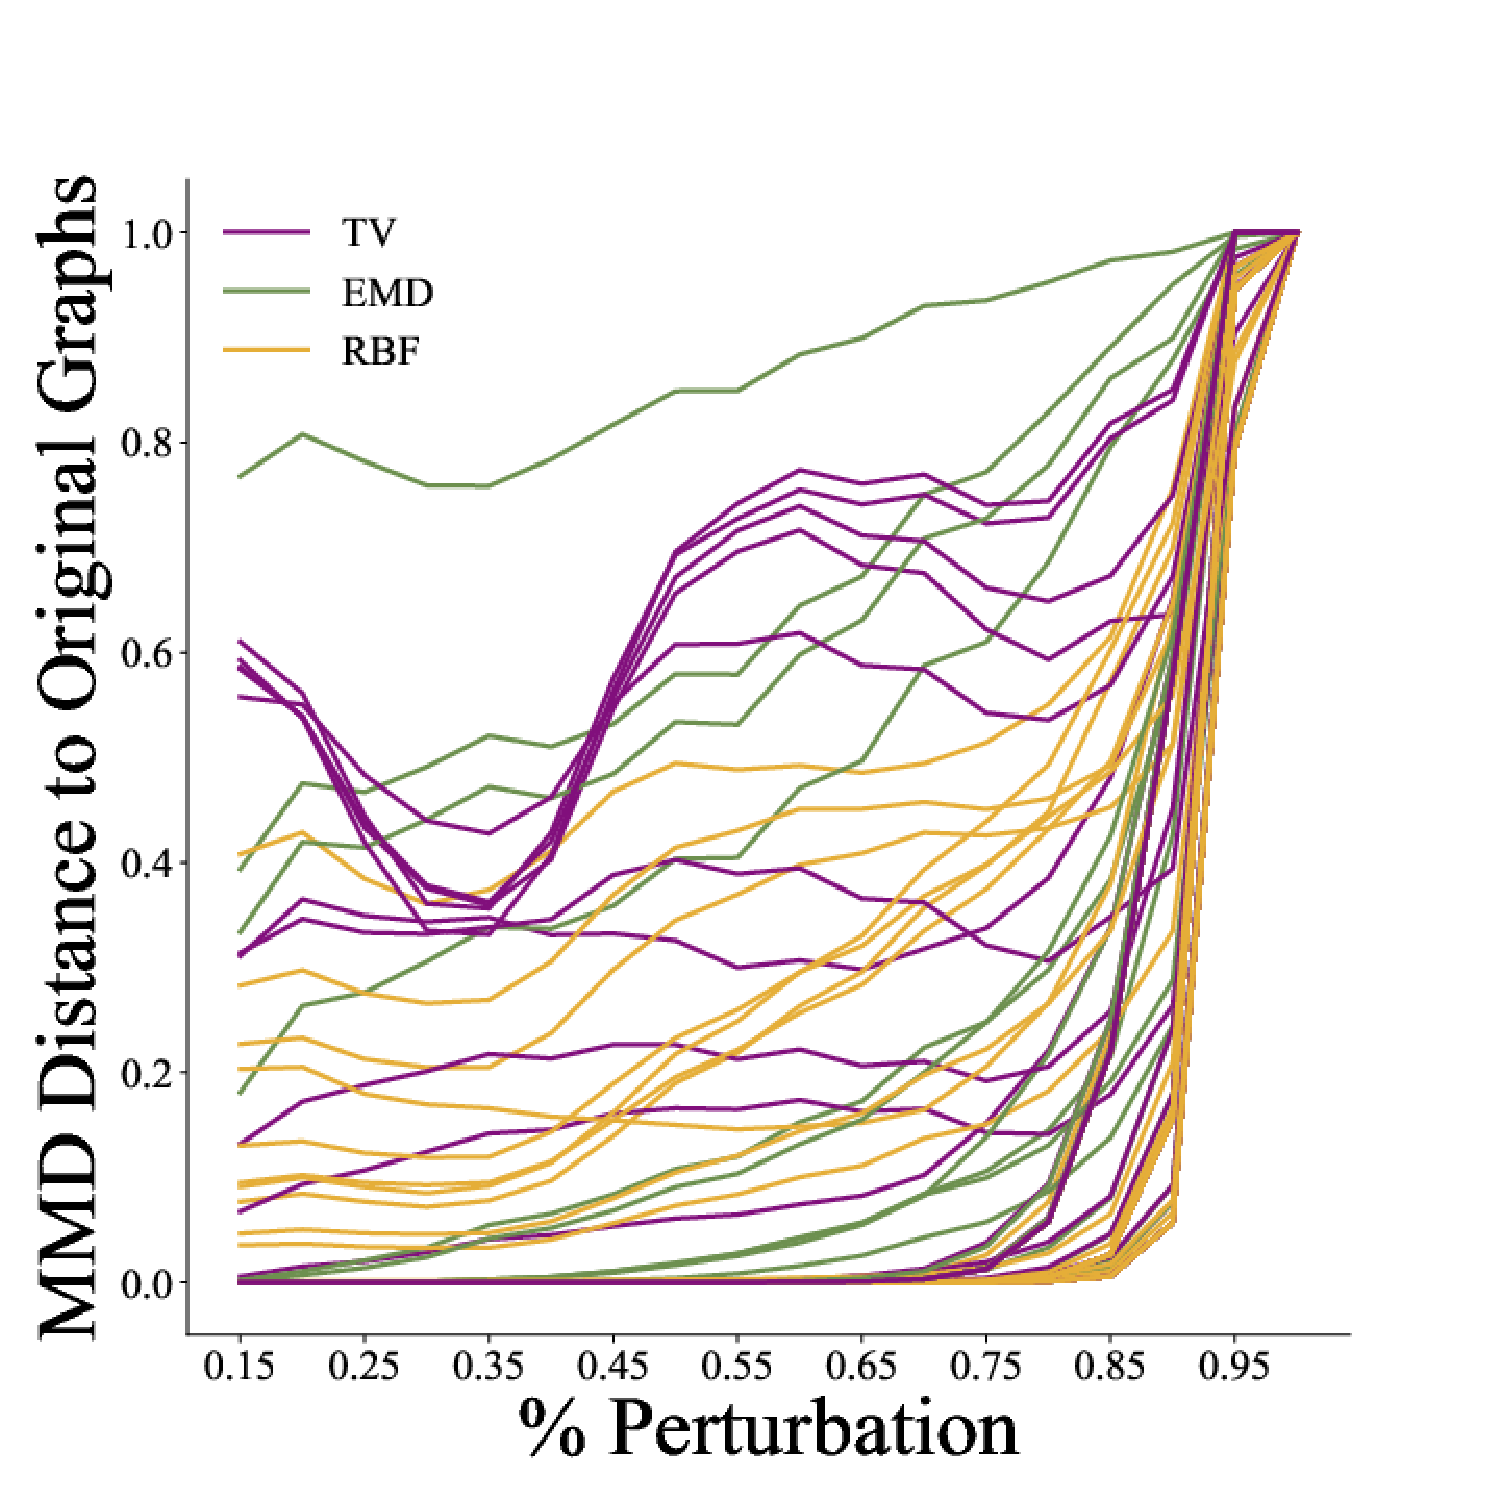
\includegraphics[width=.7\textwidth]{./figures/leslie_work.pdf}
    \caption{MMD computed from a clustering coefficient on synthetic graphs. TV:
    total variation kernel, RBF: radial basis function, EMD: earth mover's distance.}
\end{figure}
\vspace{-14pt}
  \begin{figure}
    \centering
    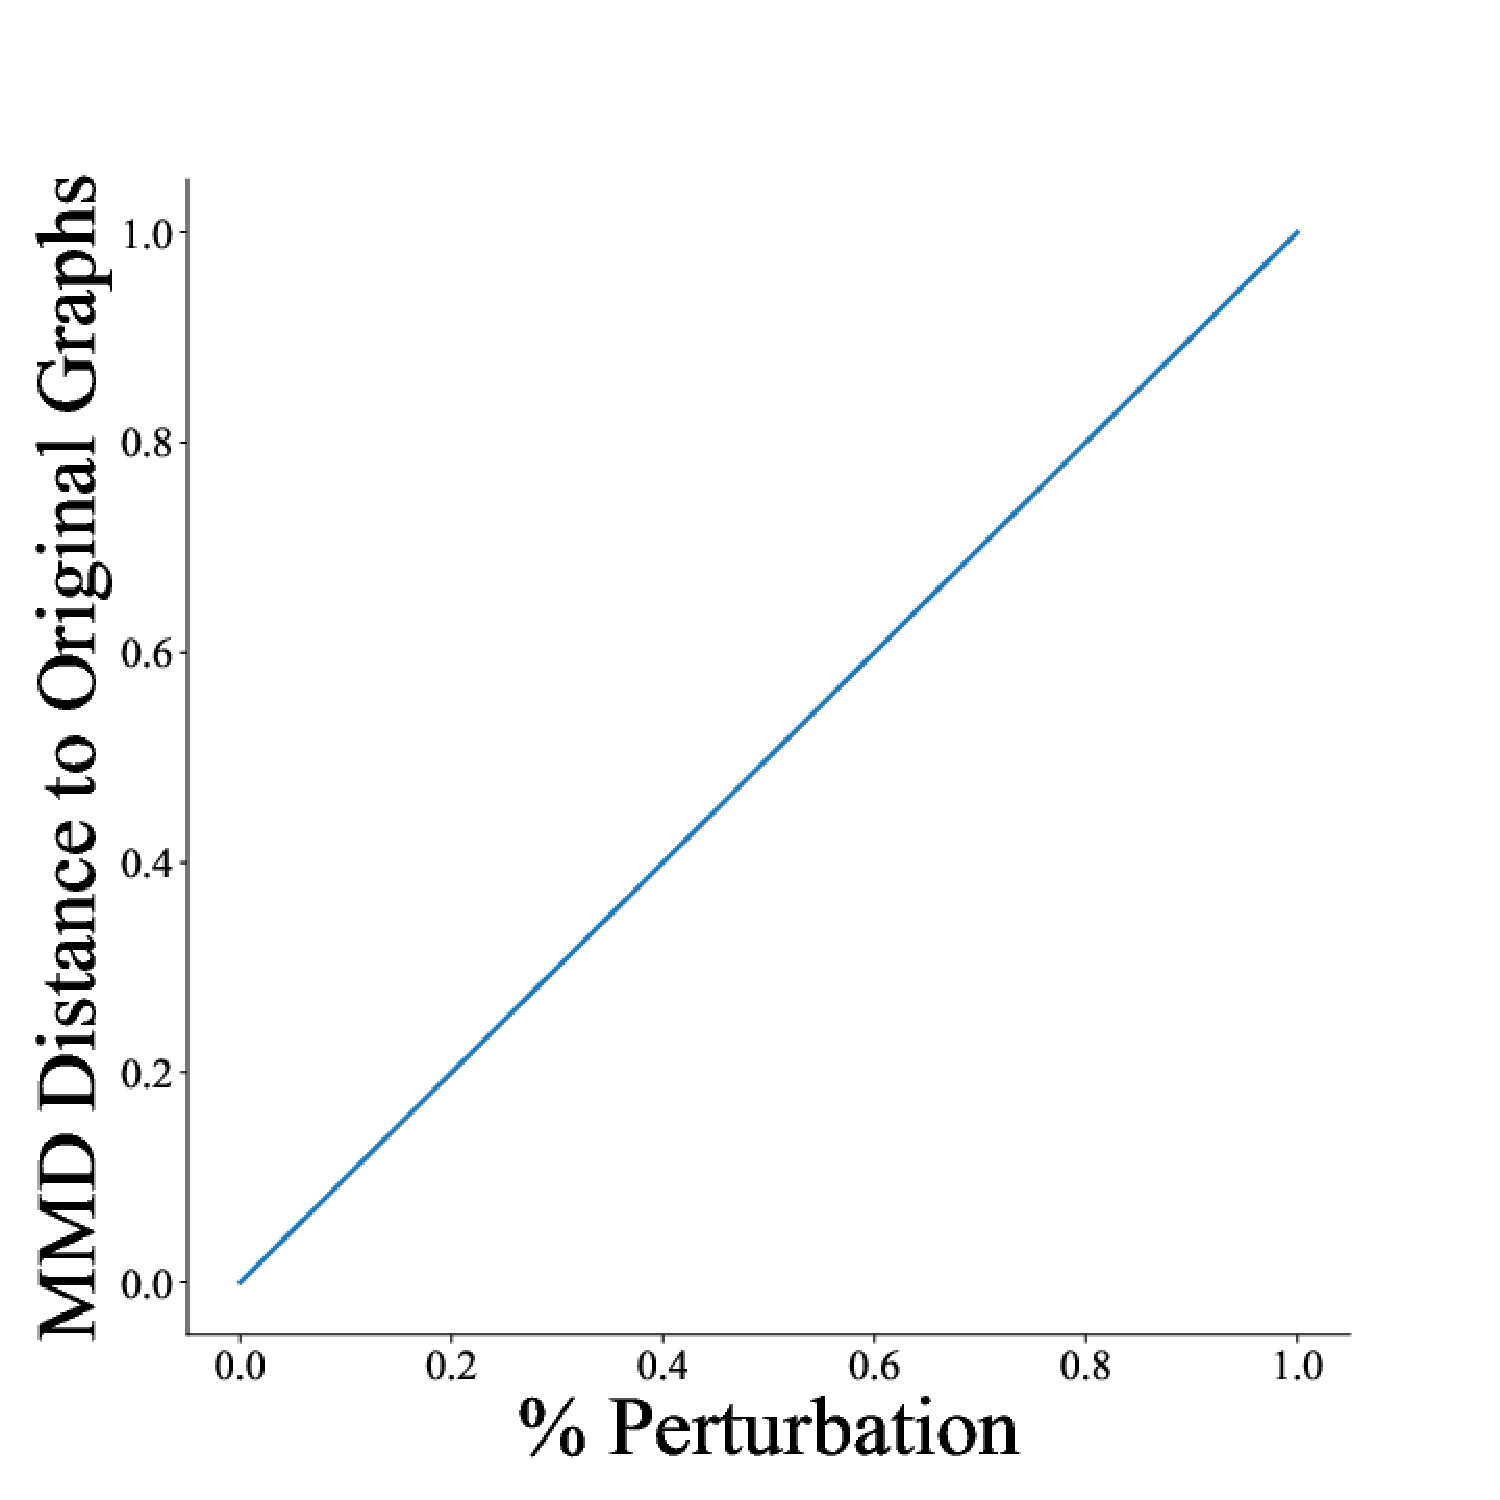
\includegraphics[width=.7\textwidth]{./figures/ideal.pdf}
    \caption{Ideal MMD behaviour.}
  \end{figure}
  \end{minipage}
\end{frame}


\begin{frame}[standout]
  -- Thesis Goal -- \\
  Build a library to evaluate generative protein models
\end{frame}

{
  \setbeamercolor{background canvas}{bg=white}
\begin{frame}[fragile]{Experimental setup}
  Take 10 sets of 100 proteins from Alphafold DB (easy to work with)
  \begin{minipage}{0.3\textwidth}
    \begin{figure}
      \centering
      % \animategraphics[loop,controls,width=0.5\linewidth]{10}{./figures/gaussian_noise/protein_straight_}{0}{49}
      \animategraphics[loop,controls,width=\linewidth]{10}{./figures/gaussian_noise/protein_straight_}{0}{1}
      \caption{Adding Gaussian Noise. Color-coded according to the index.}
      \label{fig:gaussian}
    \end{figure}
  \end{minipage}
  \hfill
  \begin{minipage}{0.3\textwidth}
    \begin{figure}
      \centering
      % \animategraphics[loop,controls,width=0.5\linewidth]{10}{./figures/gaussian_noise/protein_straight_}{0}{49}
      \animategraphics[loop,controls,width=\linewidth]{10}{./figures/twist/protein_straight_}{0}{1}
      \caption{Adding Twist. Color-coded according to the index.}
      \label{fig:twist}
    \end{figure}
  \end{minipage}
  \hfill
  \begin{minipage}{0.3\textwidth}
    \begin{figure}
      \centering
      % \animategraphics[loop,controls,width=0.5\linewidth]{10}{./figures/gaussian_noise/protein_straight_}{0}{49}
      \animategraphics[loop,controls,width=\linewidth]{10}{./figures/mutation/protein_straight_}{0}{1}
      \caption{Adding Mutations. Color-coded according to amino acid type.}
      \label{fig:mutation}
    \end{figure}
  \end{minipage}
\end{frame}
}

% {
%   \setbeamercolor{background canvas}{bg=white}
% \begin{frame}[fragile]{Experiment 1 -- Gaussian Noise}
%   \begin{figure}
%     \centering
%     \scalebox{0.75}{
%       \begin{tikzpicture}[align=center, node distance=1.5cm, align=center]
%         \node (coords) [orangebox] {Get \\Coordinates};
%         \onslide<1->\node (gauss) [orangebox, right of=coords, xshift=1.5cm, fill=PineGreen!60] {Add \\gaussian noise};
%         \draw [arrow] (coords) -- (gauss);
%         % \onslide<2-> \node (cmap) [orangebox, right of=gauss, xshift=1.5cm] {Get \\contact map};
%         % \draw [arrow] (gauss) -- (cmap);
%         % \onslide<3->\node (egraph) [orangebox, right of=cmap, xshift=1.5cm] {Get \\$\epsilon$-graph};
%         % \draw [arrow] (cmap) -- (egraph);
%         % \onslide<4->\node (wlk) [orangebox, right of=egraph, xshift=1.5cm] {Compute \\kernel};
%         % \draw [arrow] (egraph) -- (wlk);
%         % \onslide<5->\node (mmd) [orangebox, right of=wlk, xshift=1.5cm] {Compute \\MMD};
%         % \draw [arrow] (wlk) -- (mmd);
%       \end{tikzpicture}
%     }
%   \end{figure}
%   \begin{figure}
%     \centering
%     % \animategraphics[loop,controls,width=0.5\linewidth]{10}{./figures/gaussian_noise/protein_straight_}{0}{49}
%     \animategraphics[loop,controls,width=0.5\linewidth]{10}{./figures/gaussian_noise/protein_straight_}{0}{1}

%     \caption{Adding Gaussian Noise. Protein is color-coded according to the
%       index of each amino acid.}
%     \label{fig:twist}
%   \end{figure}
% \end{frame}
% }

\begin{frame}[fragile]{Experiment 1 -- Gaussian Noise \includegraphics[height=28pt]{./figures/gaussian_noise/thumbnail_protein_straight_9.png}}
  \begin{figure}
    \centering
    \scalebox{0.75}{
      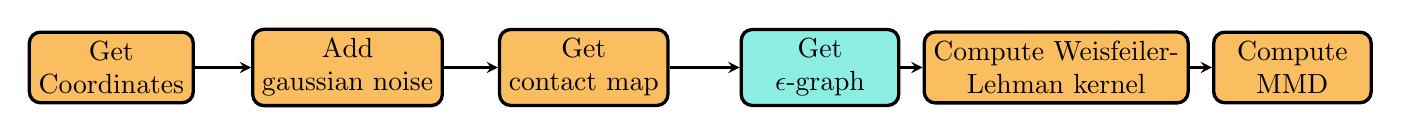
\begin{tikzpicture}[align=center, node distance=1.5cm, align=center]
        \node (coords) [orangebox] {Get \\Coordinates};
        \node (gauss) [orangebox, right of=coords, xshift=1.5cm] {Add \\gaussian noise};
        \draw [arrow] (coords) -- (gauss);
        \node (cmap) [orangebox, right of=gauss, xshift=1.5cm] {Get \\contact map};
        \draw [arrow] (gauss) -- (cmap);
        \node (egraph) [orangebox, right of=cmap, xshift=1.5cm, fill=Turquoise!60] {Get \\ $\epsilon$-graph};
        \draw [arrow] (cmap) -- (egraph);
        \node (wlk) [orangebox, right of=egraph, xshift=1.5cm] {Compute Weisfeiler-\\ Lehman kernel};
        \draw [arrow] (egraph) -- (wlk);
        \node (mmd) [orangebox, right of=wlk, xshift=1.5cm] {Compute \\MMD};
        \draw [arrow] (wlk) -- (mmd);
      \end{tikzpicture}

    }
  \end{figure}
  \pause\begin{minipage}{0.6\linewidth}
    \begin{figure}
      \centering
      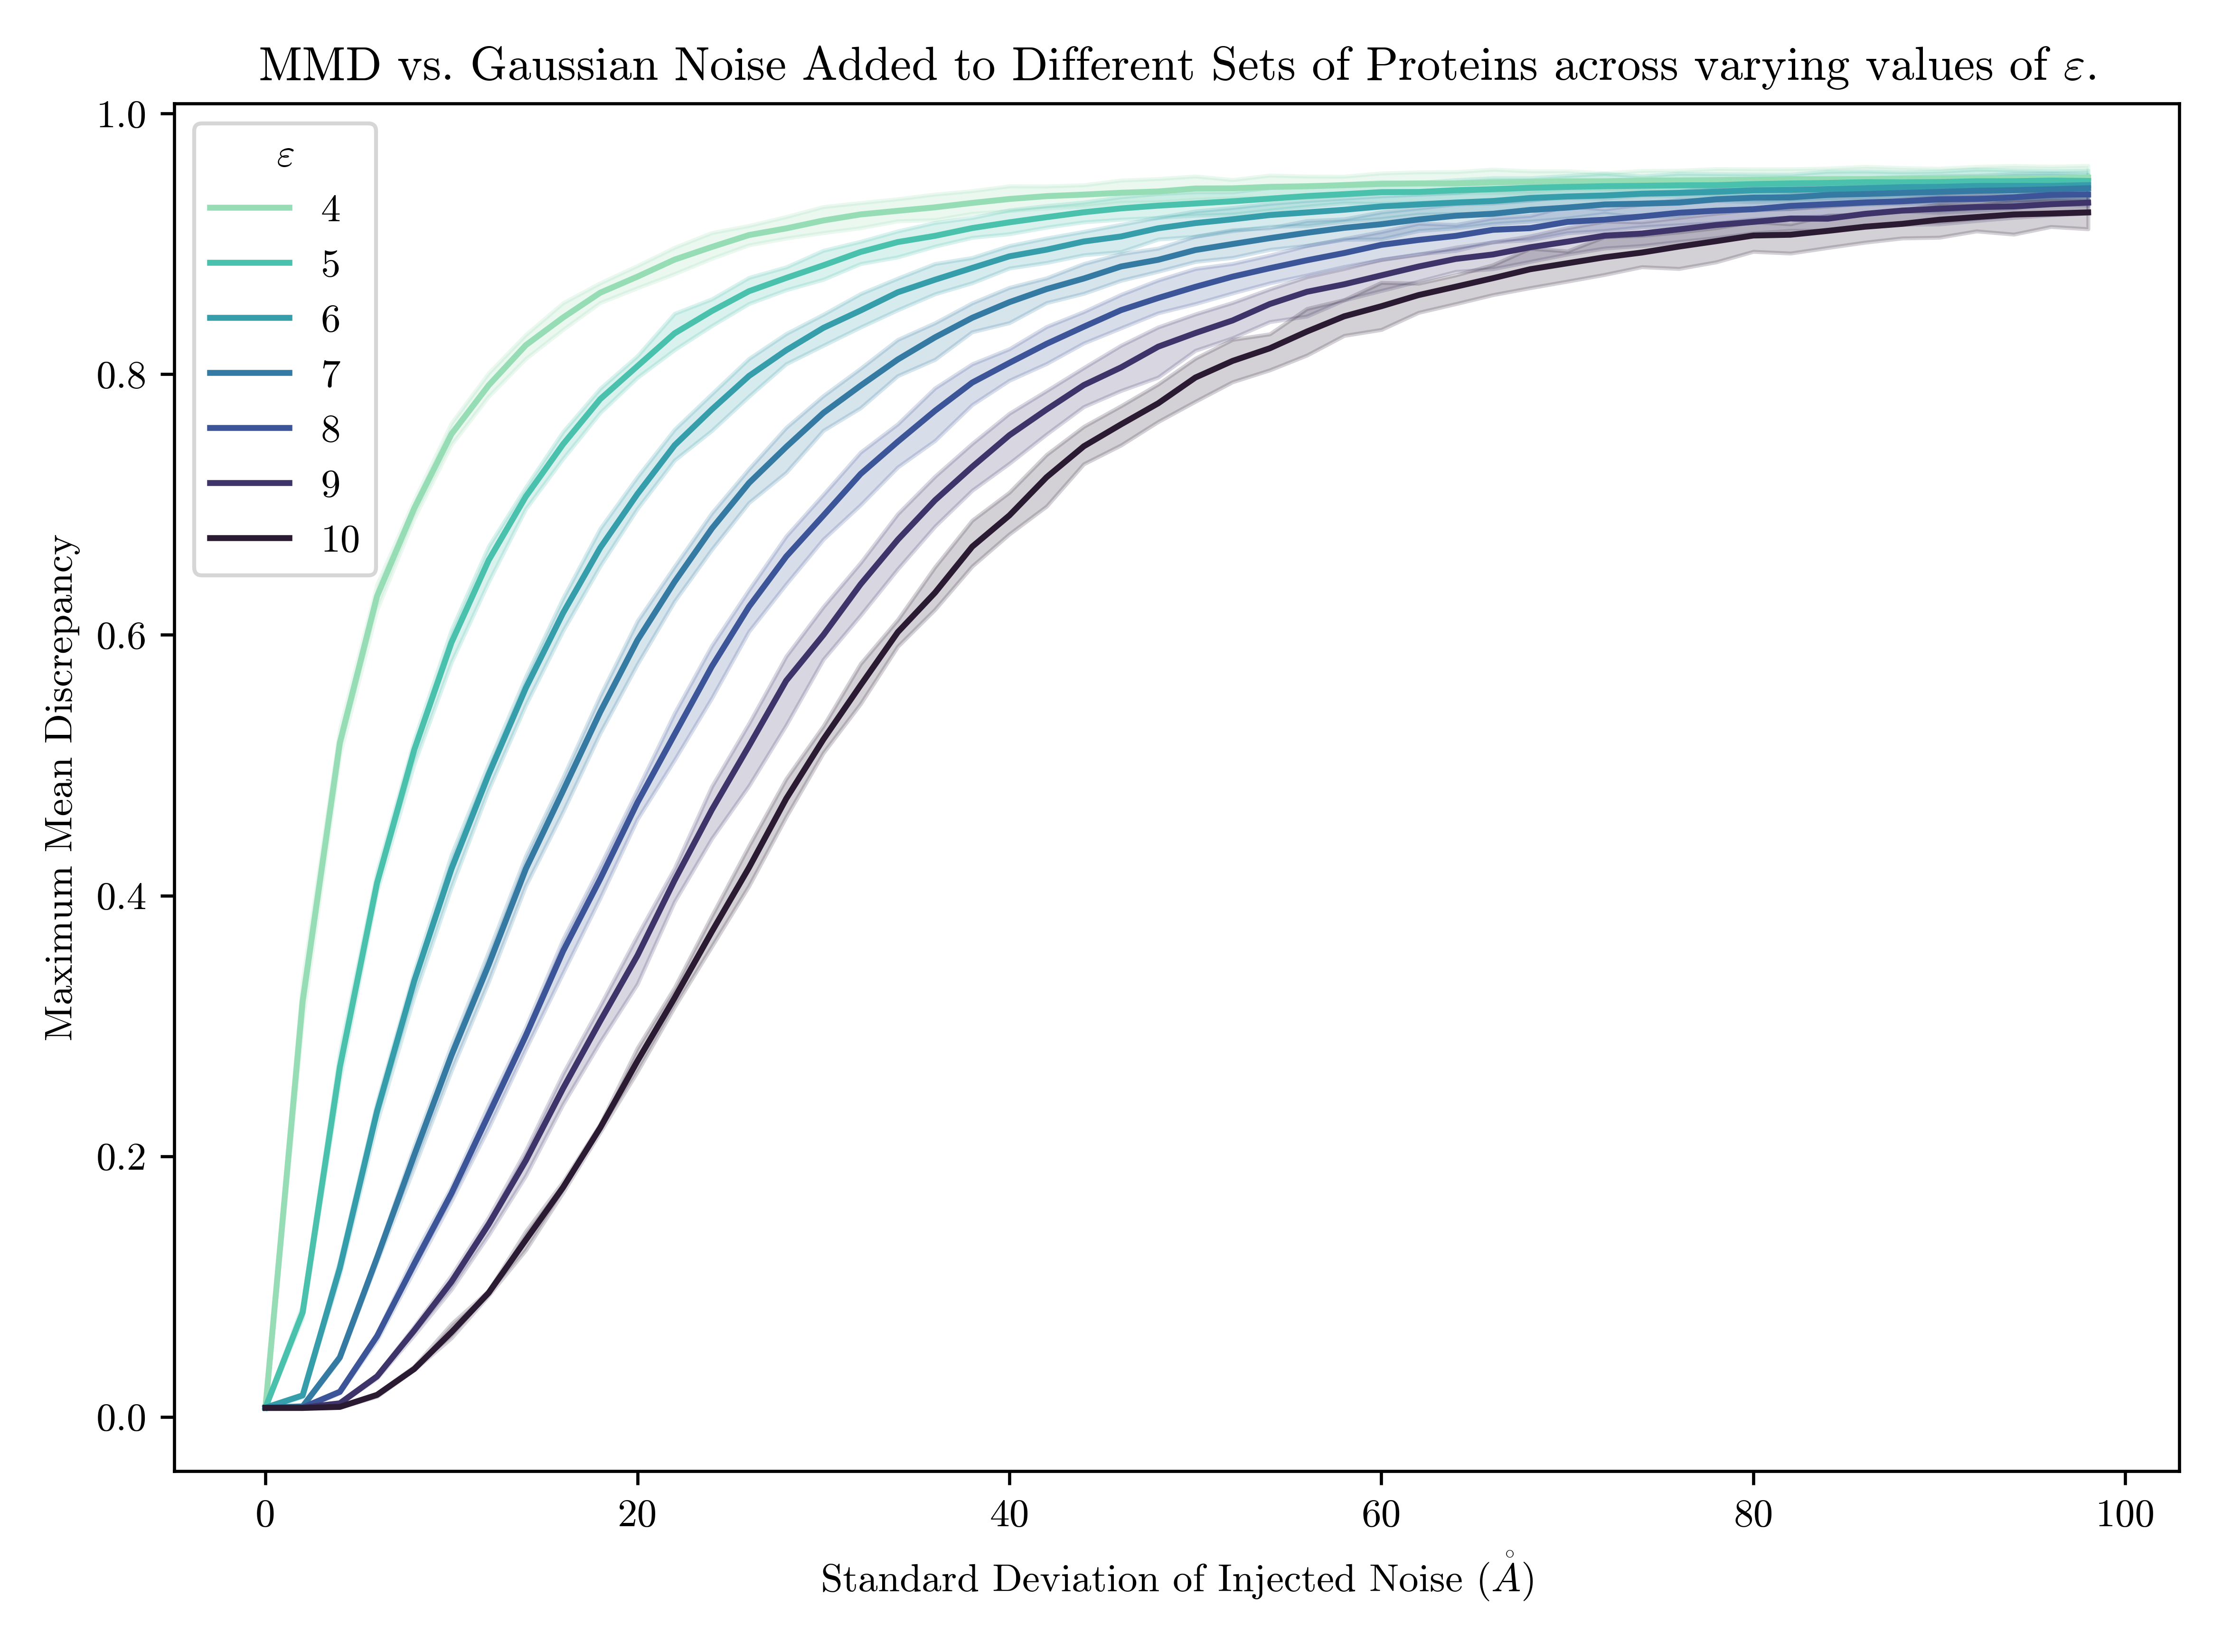
\includegraphics[width=\textwidth]{./figures/gaussian.png}
    \end{figure}
  \end{minipage}
  \begin{minipage}{0.38\linewidth}
    Each curve: different $\varepsilon$.\\

    \pause\small 2 sources of variance:
    \begin{itemize}
      \pause\small\item Data
      \pause\small\item Noise
  \end{itemize}

  \begin{alert}{Conclusions}
    \begin{enumerate}
      \pause\item MMD is stable using the Weisfeiler-Lehman kernel
      \pause\item Choice of representation influences MMD
    \end{enumerate}
  \end{alert}
  \end{minipage}
\end{frame}


{
  \setbeamercolor{background canvas}{bg=white}
  \begin{frame}[fragile]{Dihedral angles}
    \begin{minipage}{0.7\textwidth}
      \begin{figure}
        \centering
        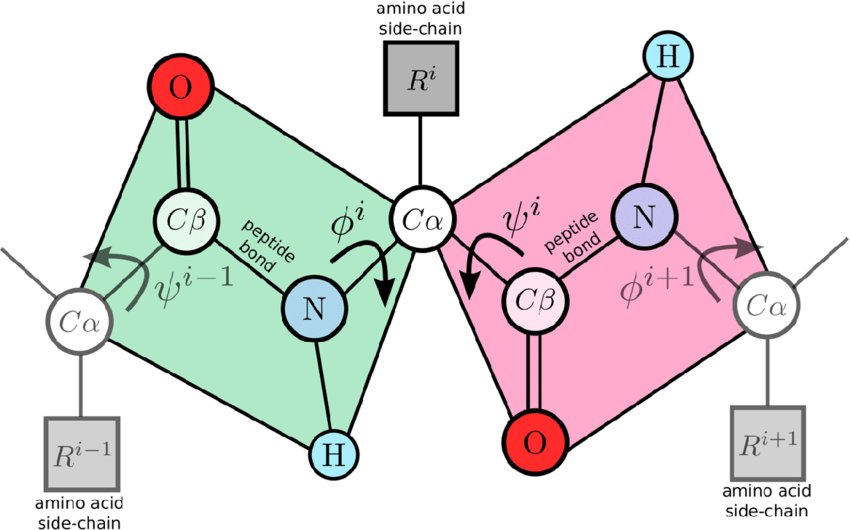
\includegraphics[width=\textwidth]{./figures/phi_psi.png}
      \end{figure}
    \end{minipage}
    \hfill
    \begin{minipage}{0.25\textwidth}
      \small These angles \emph{define} the shape of the protein.
    \end{minipage}
  \end{frame}
}


\begin{frame}[fragile]{\v{C}ech filtrations}
  \begin{minipage}{0.7\textwidth}
    \begin{figure}
      \centering
      \animategraphics[loop,controls,width=0.5\linewidth]{10}{./figures/cech_filtration/something-}{0}{149}%
% \animategraphics[loop,controls,width=0.5\linewidth]{10}{./figures/cech_filtration/something-}{0}{1}
      \label{fig:cech}
    \end{figure}
  \end{minipage}
  \hfill
  \begin{minipage}{0.25\textwidth}
    \small \v{C}ech filtrations captures connected components, cycles and holes
    by varying $\varepsilon$.
  \end{minipage}
\end{frame}

{
  \setbeamercolor{background canvas}{bg=white}
  \begin{frame}[fragile]{Experiment 2 -- Twist}
    \begin{minipage}{0.58\textwidth}

  \begin{figure}
    \centering
    \scalebox{0.55}{
    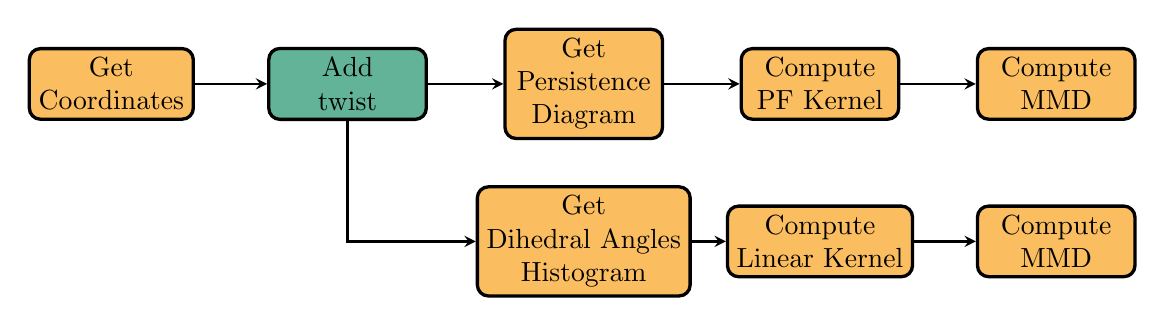
\begin{tikzpicture}[align=center, node distance=1.5cm, align=center]
      \node (coords) [orangebox] {Get \\Coordinates};
      \node (twist) [orangebox, right of=coords, xshift=1.5cm, fill=PineGreen!60] {Add \\twist};
      \draw [arrow] (coords) -- (twist);
      \node (pd) [orangebox, right of=twist, xshift=1.5cm] {Get \\Persistence \\Diagram};
      \draw [arrow] (twist) -- (pd);
      \node (wlk) [orangebox, right of=pd, xshift=1.5cm] {Compute \\PF Kernel};
      \draw [arrow] (pd) -- (wlk);
      \node (mmd) [orangebox, right of=wlk, xshift=1.5cm] {Compute \\MMD};
      \draw [arrow] (wlk) -- (mmd);
      \node (rama) [orangebox, below of=pd, yshift=-0.5cm] {Get \\Dihedral Angles\\ Histogram};
      \draw [arrow] (twist) |- (rama);
      \node (lin) [orangebox, right of=rama, xshift=1.5cm] {Compute \\Linear Kernel};
      \draw [arrow] (rama) -- (lin);
      \node (mmdlin) [orangebox, right of=lin, xshift=1.5cm] {Compute \\MMD};
      \draw [arrow] (lin) -- (mmdlin);
    \end{tikzpicture}
    }
  \end{figure}
\end{minipage}
\hfill
\begin{minipage}{0.38\textwidth}
  \begin{figure}
    \centering
    \animategraphics[loop,controls,width=\textwidth]{10}{./figures/twist/protein_straight_}{0}{99}
    % \animategraphics[loop,controls,width=0.4\linewidth]{10}{./figures/twist/protein_straight_}{0}{1}
    % \caption{Adding Gaussian Noise. Protein is color-coded according to the
    % index of each amino acid.}
    \label{fig:twist}
  \end{figure}
\end{minipage}
\end{frame}
}

  {
  \setbeamercolor{background canvas}{bg=white}
\begin{frame}[fragile]{Experiment 2 -- Twist}
  \begin{minipage}{0.6\linewidth}
    \begin{figure}
      \centering
      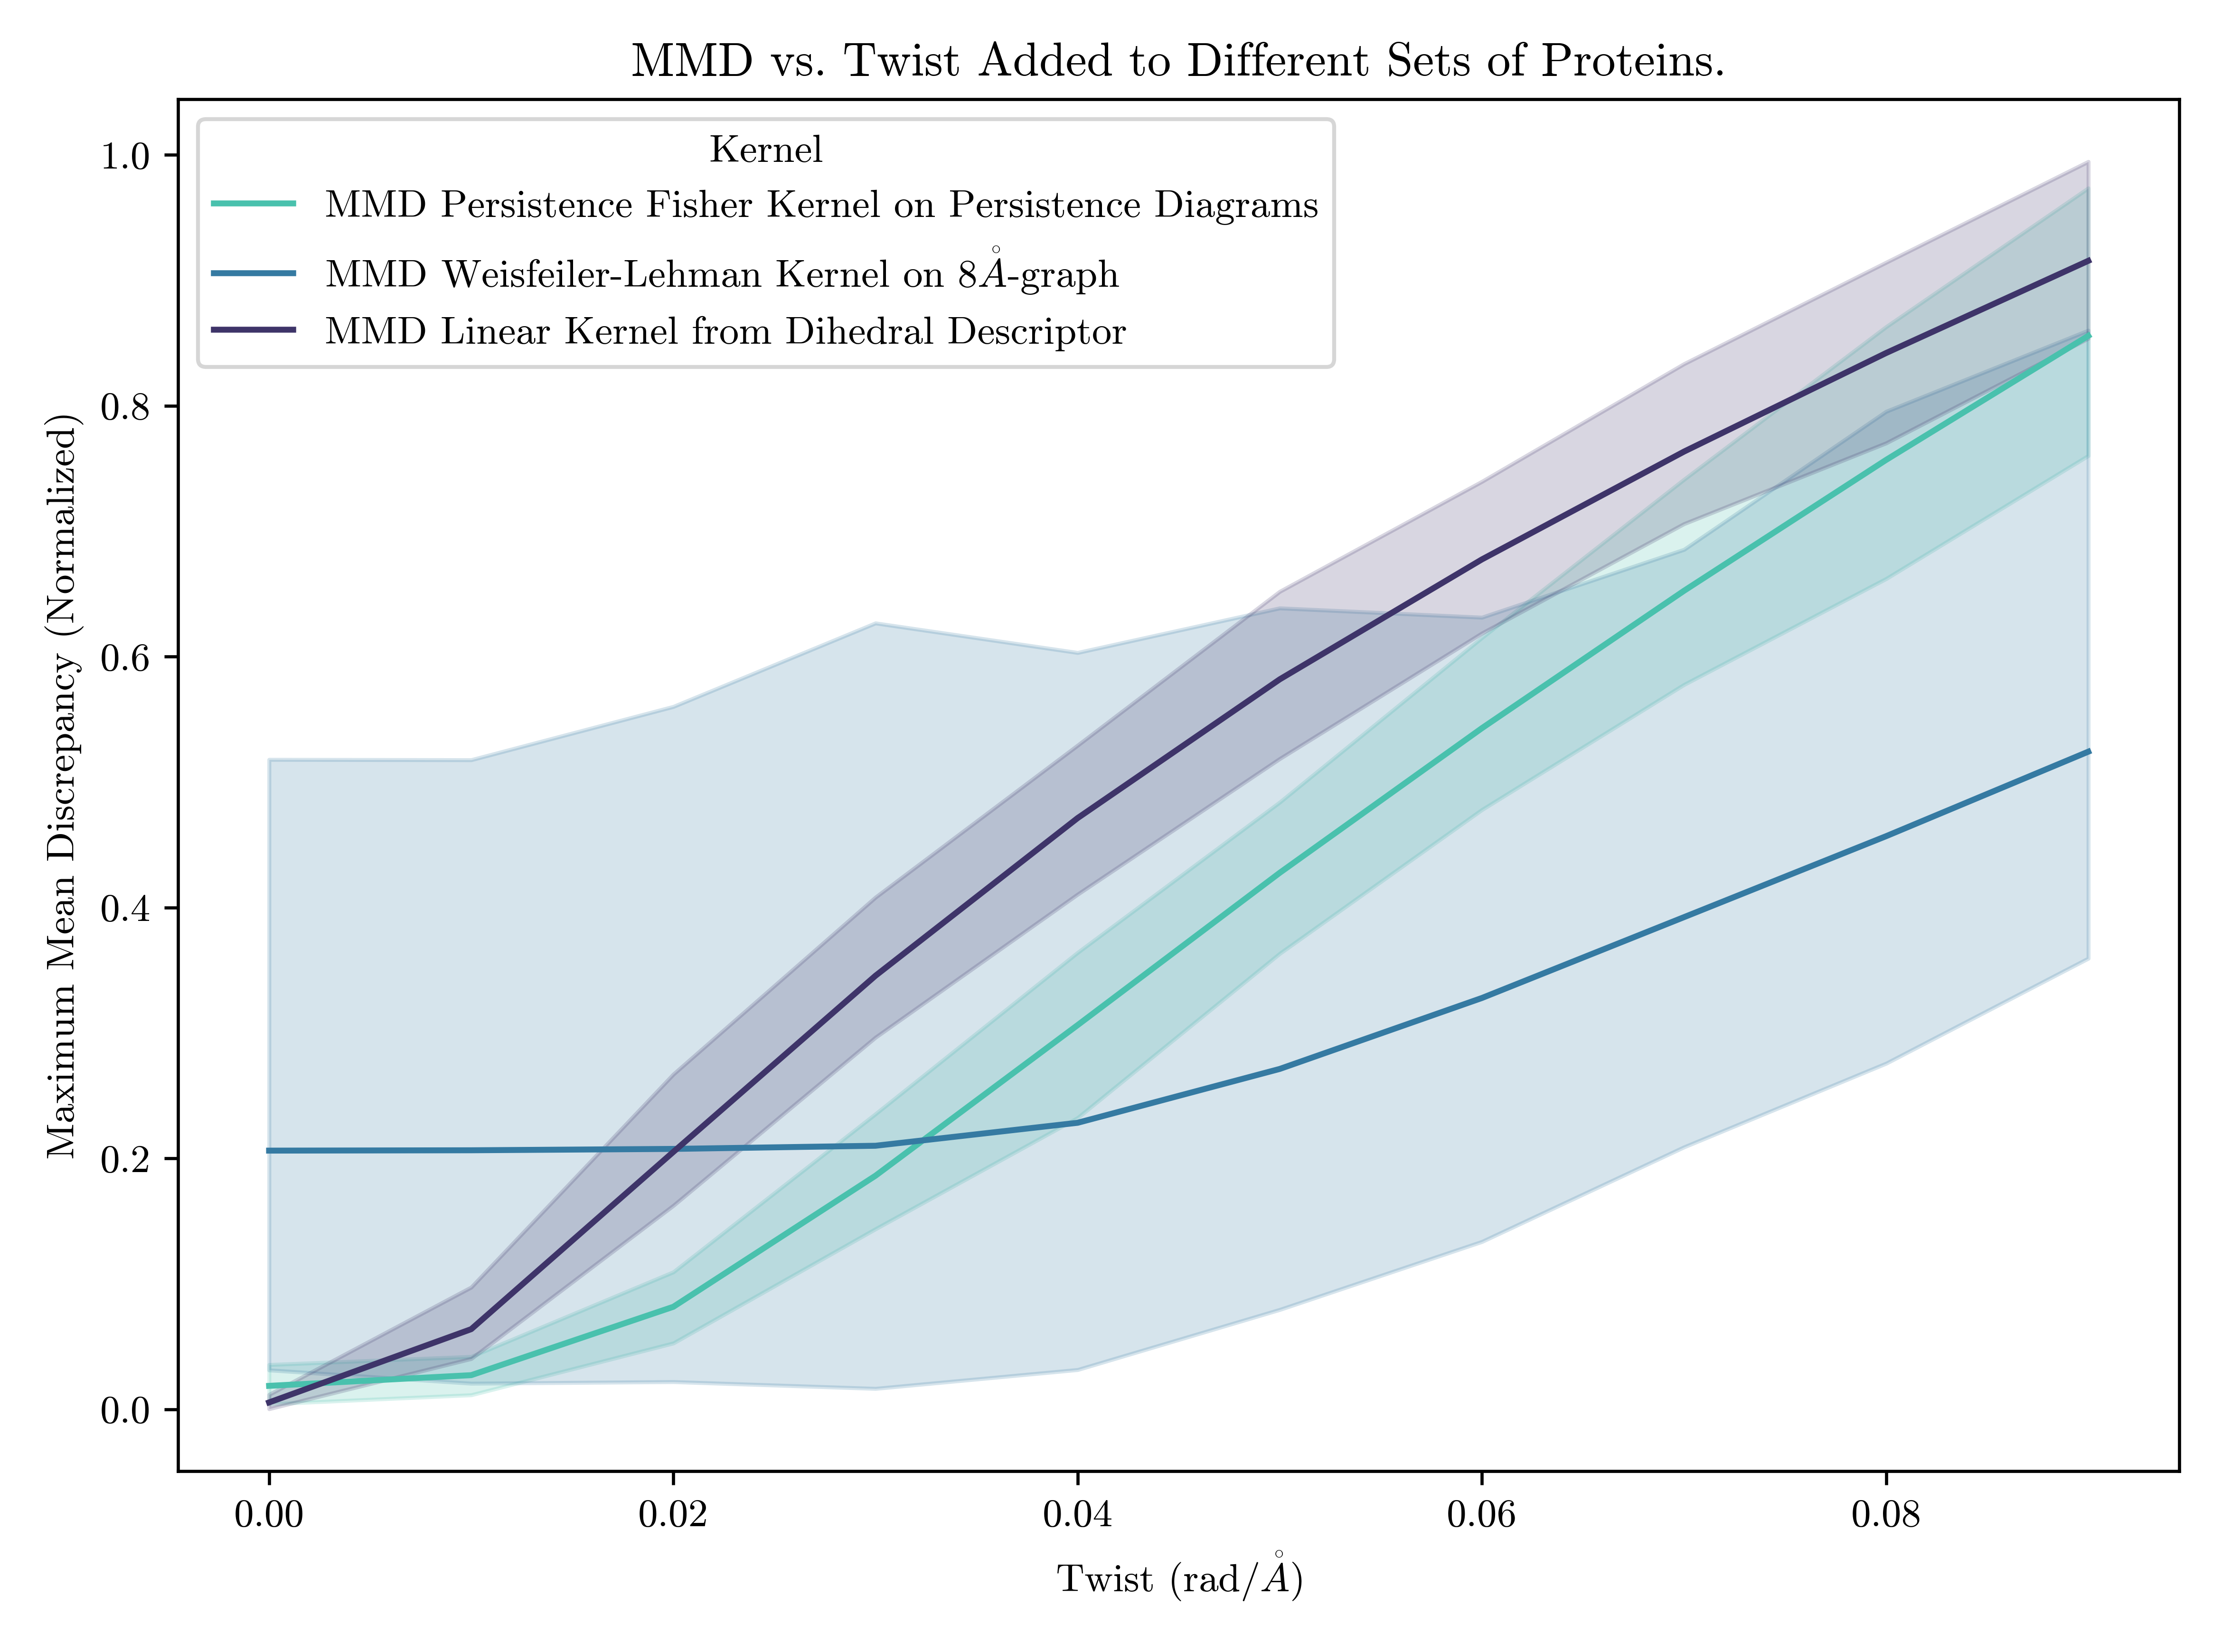
\includegraphics[width=\textwidth]{./figures/twist.png}
    \end{figure}
  \end{minipage}
  \begin{minipage}{0.38\linewidth}

    \pause\small 1 source of variance:
    \begin{itemize}
      \pause\small\item Data
  \end{itemize}

  \begin{alert}{Conclusions}
    \begin{enumerate}
      \pause\item TDA behaves very well, computationally complex
      \pause\item Dihedral descriptor behave well, fast to compute
      \pause\item Weisfeiler-Lehman kernel does not capture global shape changes
    \end{enumerate}
  \end{alert}
  \end{minipage}
\end{frame}
}


{
  \setbeamercolor{background canvas}{bg=white}
\begin{frame}[fragile]{Experiment 3 -- Mutate}
  \begin{figure}
    \centering
    \scalebox{0.75}{
      \begin{tikzpicture}[align=center, node distance=1.5cm, align=center]
        \node (seq) [orangebox] {Get \\Sequence};
        \node (mutate) [orangebox, right of=seq, xshift=1.5cm, fill=PineGreen!60] {Add \\mutation};
        \draw [arrow] (coords) -- (mutate);
        \node (esm) [orangebox, right of=mutate, xshift=1.5cm] {Get \\ ESM embedding};
        \draw [arrow] (mutate) -- (esm);
        \node (lin) [orangebox, right of=esm, xshift=1.5cm] {Compute \\ Linear Kernel};
        \draw [arrow] (esm) -- (lin);
        \node (mmd) [orangebox, right of=lin, xshift=1.5cm] {Compute \\MMD};
        \draw [arrow] (lin) -- (mmd);
      \end{tikzpicture}
    }
  \end{figure}
 \end{frame}
}

{
  \setbeamercolor{background canvas}{bg=white}
\begin{frame}[fragile]{Experiment 3 -- Mutate}
 \begin{minipage}{0.6\linewidth}
    \begin{figure}
      \centering
      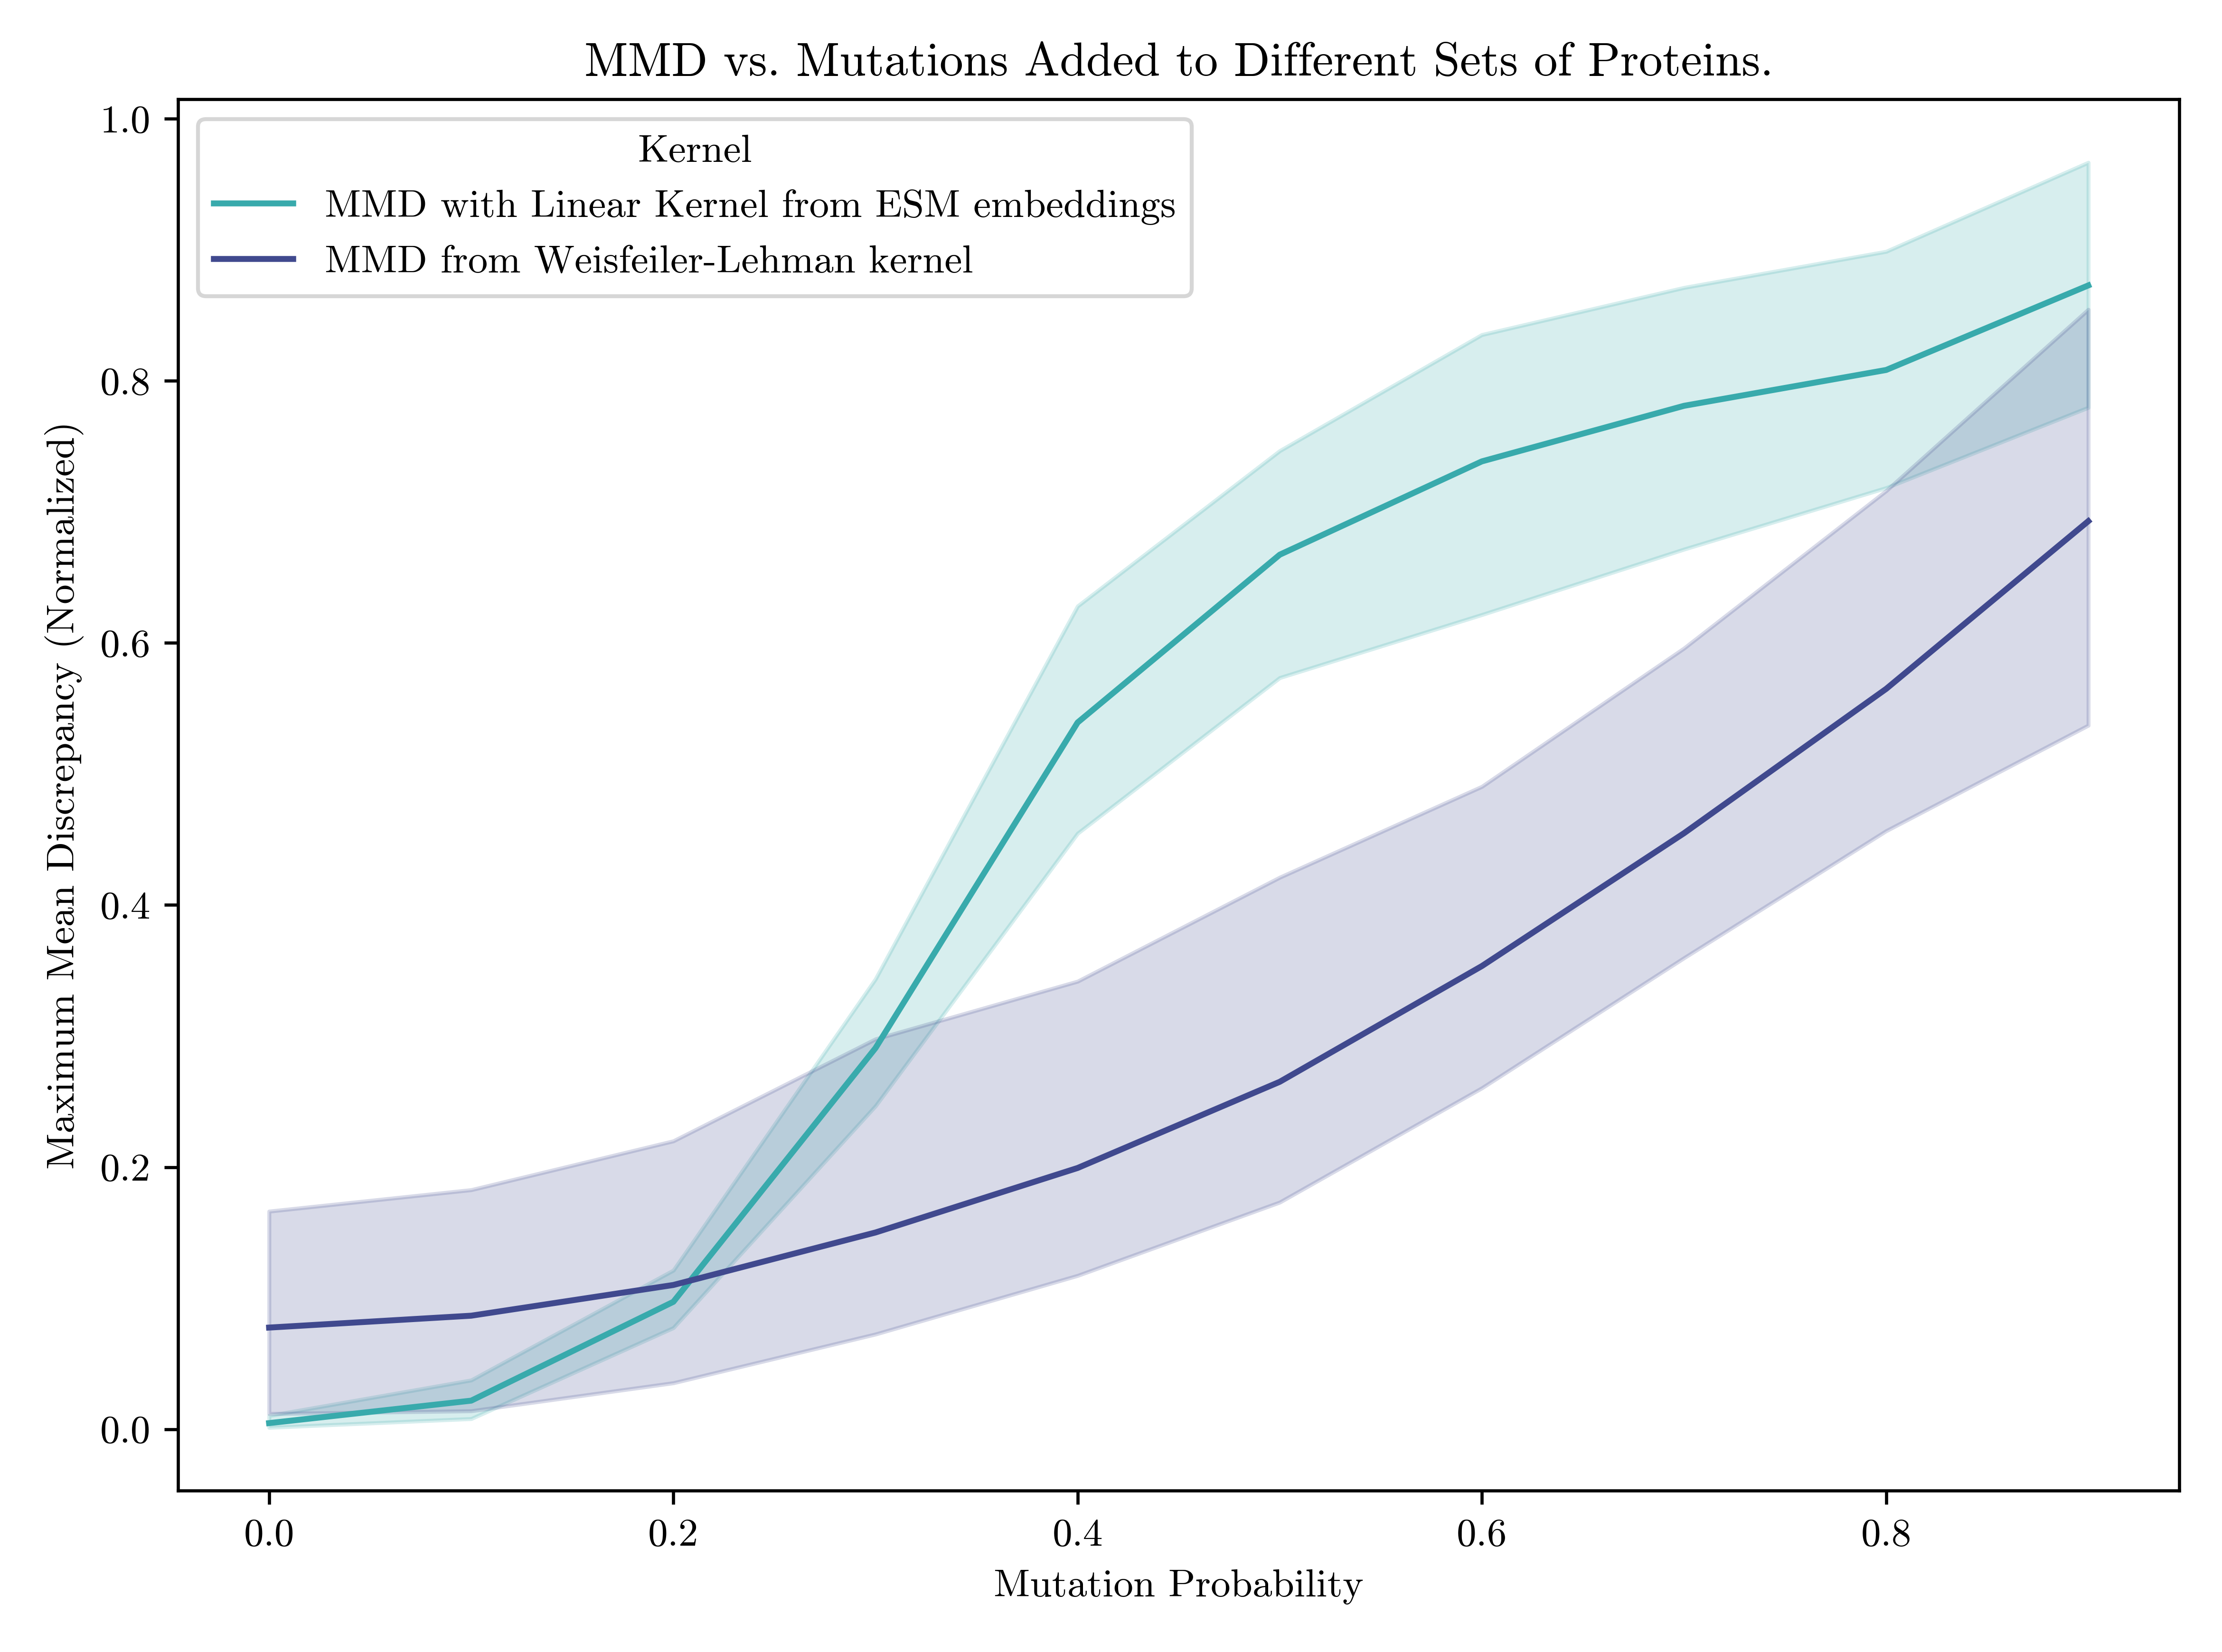
\includegraphics[width=\textwidth]{./figures/mutation.png}
    \end{figure}
  \end{minipage}
  \begin{minipage}{0.38\linewidth}
    % \pause $n=10$ runs

    \pause\small 2 sources of variance:
    \begin{itemize}
      \pause\small\item Data
      \pause\small\item Mutation seed
  \end{itemize}

  \pause\begin{alert}{Conclusions}
    \begin{enumerate}
      \pause\item Weisfeiler-Lehman kernel captures changes but noisy
      \pause\item ESM captures changes.
      \pause\item Further study with lower mutation probabilities.
    \end{enumerate}
  \end{alert}
  \end{minipage}
\end{frame}
}

\begin{frame}[fragile]{Questions - Overview}
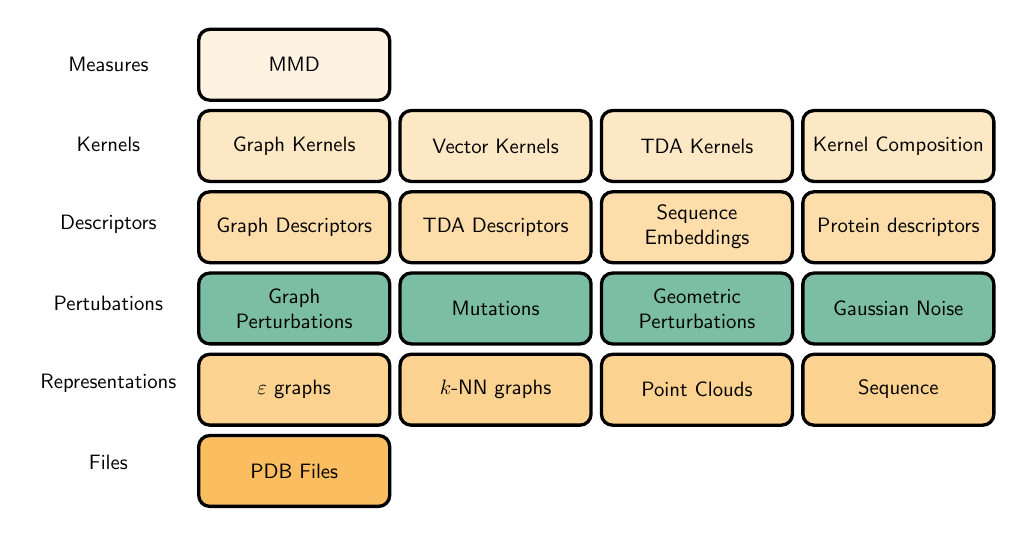
\begin{tikzpicture}[
	scale=0.75,
	start chain=1 going below,
	start chain=2 going right,
	node distance=1mm,
	desc/.style={
		scale=0.75,
		on chain=2,
		rectangle,
		rounded corners,
		draw=black,
		very thick,
		text centered,
		text width=3cm,
		minimum height=12mm,
		fill=blue!30
  },
	it/.style={
		fill=blue!10
	},
	level/.style={
		scale=0.75,
		on chain=1,
		minimum height=12mm,
		text width=2.5cm,
		text centered,
	},
	every node/.style={font=\sffamily}
]

\node [level] (Level 5) {Measures};
\node [level] (Level 4) {Kernels};
\node [level] (Level 3) {Descriptors};
\node [level] (Level 2) {Pertubations};
\node [level] (Level 1) {Representations};
\node [level] (Level 0) {Files};

\chainin (Level 5);
\node [desc, fill=YellowOrange!10] (mmd) {MMD};
\node [desc, continue chain=going below, fill=YellowOrange!20] (gkernels) {Graph Kernels};
\begin{scope}[start branch=gkernels]
  \node[desc, on chain=going right, fill=YellowOrange!20](vkernels) {Vector Kernels};
  \node[desc, on chain=going right, fill=YellowOrange!20](tdakernels) {TDA Kernels};
  \node[desc, on chain=going right, fill=YellowOrange!20](tdakernels) {Kernel Composition};
\end{scope}
\node [desc, fill=YellowOrange!30] (gdescriptors) {Graph Descriptors};
\begin{scope}[start branch=gdescriptors]
  \node[desc, fill=YellowOrange!30, on chain=going right](tdadescriptors) {TDA Descriptors};
  \node[desc, on chain=going right, fill=YellowOrange!30](sequence) {Sequence \\Embeddings};
  \node[desc, on chain=going right, fill=YellowOrange!30](sequence) {Protein descriptors};
\end{scope}
\node [desc, xshift=2.25cm, xshift=-2.25cm, fill=PineGreen!50] (pert) {Graph \\Perturbations};
\begin{scope}[start branch= pert]
  \node[desc, on chain=going right, fill=PineGreen!50](gp) {Mutations};
  \node[desc, on chain=going right, fill=PineGreen!50](gp) {Geometric \\Perturbations};
  \node[desc, on chain=going right, fill=PineGreen!50](gn) {Gaussian Noise};
\end{scope}
\node [desc, fill=YellowOrange!40] (Graphs) {$\varepsilon$ graphs};
\begin{scope}[start branch=Graphs]
  \node[desc, on chain=going right, fill=YellowOrange!40](knn) {$k$-NN graphs};
  \node[desc, on chain=going right, fill=YellowOrange!40] (PC) {Point Clouds};
  \node[desc, on chain=going right, fill=YellowOrange!40] (Seq) {Sequence};
\end{scope}
\node [desc, fill=YellowOrange!60] (Files) {PDB Files};
\end{tikzpicture}
\end{frame}





\begin{frame}[fragile]{Maximum Mean Discrepancy (MMD)}
  \begin{equation*}
    \text{MMD}(X, Y) := {1\over n^2} \sum_{i,j=1}^{n}k(x_i, x_j) + {1\over m^2} \sum_{i,j=1}^{n}k(y_i, y_j) - {2\over nm} \sum_{i=1}^{n}\sum_{j=1}^{m}k(x_i, y_j)
  \end{equation*}
    where:
    \begin{itemize}
    \item $\mathcal{X}$ is some non-empty set.
    \item  $x_i, x_j \subseteq \mathcal{X}$, $n$ is the number of samples in $\mathbf{x}$;
    \item  $y_i, y_j \subseteq \mathcal{X}$, $m$ is the number of samples in $\mathbf{y}$;
    \item $k: \mathcal{X}\times\mathcal{X}\to\mathbb{R}$ is a valid kernel.
    \end{itemize}

    \small MMD captures the distance between 2 sets on \emph{any} RKHS $\mathcal{H}$.
  \end{frame}

{
  \setbeamercolor{background canvas}{bg=white}
  \begin{frame}[fragile]{API}
    \begin{minipage}{.45\textwidth}
      \inputminted[firstline=1, lastline=15]{python}{example_pipeline_with_noise.py}
    \end{minipage}
    \hfill
    \pause
    \begin{minipage}{.45\textwidth}
      \inputminted[firstline=17, lastline=26]{python}{example_pipeline_with_noise.py}
    \end{minipage}
  \end{frame}

  \begin{frame}[fragile]{MMD with 8-$\mathring{A}$-MMD with Weisfeiler-Lehman kernel}
    \begin{figure}
      \centering
      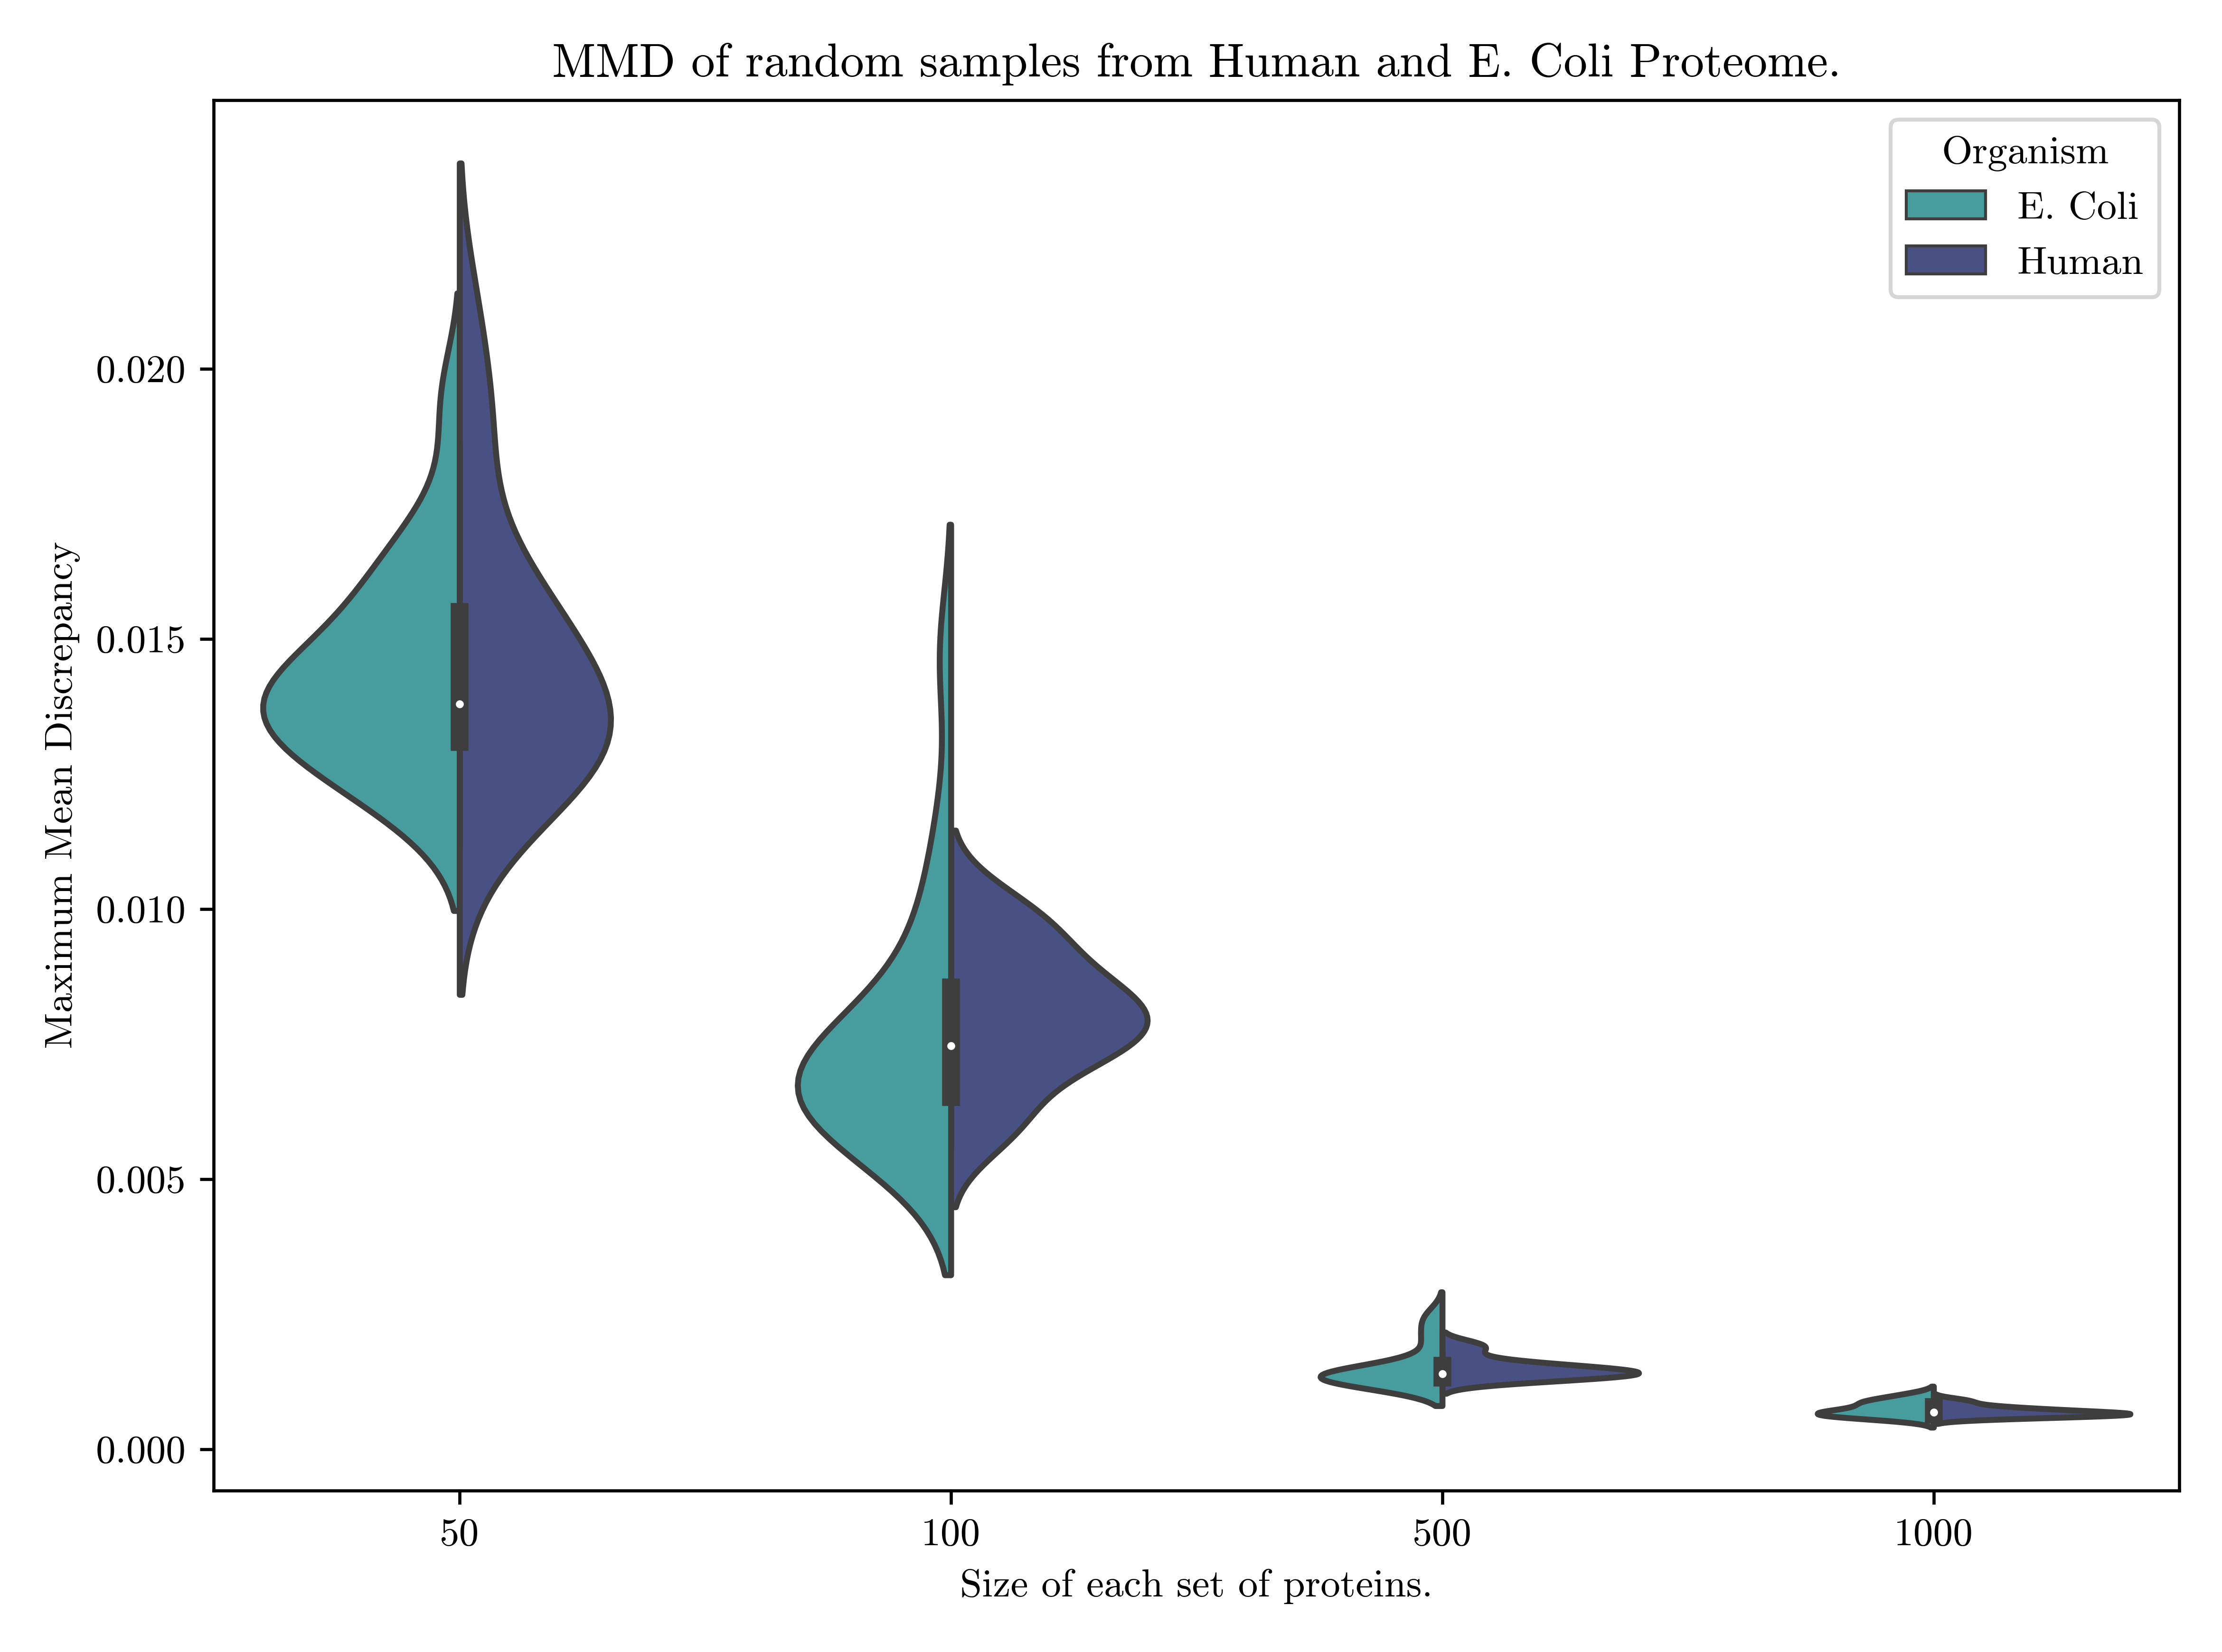
\includegraphics[height=\textheight]{./figures/mmd_variance_baseline.png}
    \end{figure}
  \end{frame}
}

\end{document}
